% ======================= Pre-Amble =========================
      
%Format
\documentclass[11pt, oneside]{article}   	% use "amsart" instead of "article" for AMSLaTeX format 
                     						%imports package {article} and specify option(s) [11pt, oneside]
\usepackage{geometry}                		% See geometry.pdf to learn the layout options. There are lots. 
    \geometry{letterpaper}                   		% ... or a4paper or a5paper or ... 
    %\geometry{landscape}                		% Activate for rotated page geometry

\usepackage[parfill]{parskip}    		        % Activate to begin paragraphs with an empty line rather than an indent

    %Colours
    \usepackage{graphicx, subcaption}
    \usepackage[usenames, dvipsnames]{color}     % font colour:    \textcolor{<colour>}{text}
          									%highlight text:  \colorbox{<color>}{text}
    \usepackage{soul}						%highlight text: \hl{}     %only  yellow								
    									%list of colours: https://www.sharelatex.com/learn/Using_colours_in_LaTeX
    									
    %Bullets
    \usepackage{enumerate}     %specify type of enumeration: \being{enumerate}[<type of enumeration>]
    
    %Footnote Spacing
    \setlength{\footnotesep}{0.4cm}                  %specify spacing b/w footnotes
    \setlength{\skip\footins}{0.6cm}                    % space b/w footnotes and textbody

	%Sections
%	\makeatletter
%	% we use \prefix@<level> only if it is defined
%	\renewcommand{\@seccntformat}[1]{
%	  \ifcsname prefix@#1\endcsname
%	    \csname prefix@#1\endcsname
%	  \else
%	    \csname the#1\endcsname\quad 
%	  \fi}
%	% define \prefix@section
%	\newcommand\prefix@section{Question \thesection}
%	\makeatother

%	\makeatletter
%	\def\@seccntformat#1{%
%	  \expandafter\ifx\csname c@#1\endcsname\c@section
%	  Question \thesection
%	  \else
%	  \csname the#1\endcsname\quad
%	  \fi}
%	\makeatother



%Mattematics
    %American Mathematics Society packages
    \usepackage{amsmath}	   %math
    \usepackage{amssymb}       %symbols
    \usepackage{amsthm}          %theorems
    \newtheorem{proposition}{Proposition}

    %QED
    \newcommand*{\QEDA}{\hfill\ensuremath{\blacksquare}}         %make qed filled square:    \QEDA
    \newcommand*{\QEDB}{\hfill\ensuremath{\square}}               %make qed empty square: \QEDB 
    \renewcommand\qedsymbol{\ensuremath{\blacksquare}}		%Proof environment
    
    % Proofs
	\newtheorem{thm}{Theorem}[section]
	\newtheorem{lem}[thm]{Lemma}
	\newtheorem{prop}[thm]{Proposition}
	\newtheorem*{cor}{Corollary}
	
	\theoremstyle{definition}
	\newtheorem{defn}{Definition}[section]
	\newtheorem{conj}{Conjecture}[section]
	\newtheorem{exmp}{Example}[section]
	
	\theoremstyle{remark}
	\newtheorem*{rem}{Remark}
	\newtheorem*{note}{Note}
	
	% Symbol Shortcuts
	\newcommand{\R}{\ensuremath{\mathbb{R}}}
	\newcommand{\C}{\ensuremath{\mathbb{C}}}
	\newcommand{\Z}{\ensuremath{\mathbb{Z}}}
	\newcommand{\Q}{\mathbb{Q}}
	\newcommand{\N}{\mathbb{N}}
	\newcommand\floor[1]{\lfloor#1\rfloor}
\newcommand\ceil[1]{\lceil#1\rceil}
	
	% Augmented Matrix
	\makeatletter
	\renewcommand*\env@matrix[1][*\c@MaxMatrixCols c]{%
  	\hskip -\arraycolsep
 		 \let\@ifnextchar\new@ifnextchar
 		 \array{#1}}
	\makeatother
	
    %\numberwithin{counterA}{counterB} 	% replaces counterA by counterb.countera
	%\numberwithin{equation}{question} 	% for equations: (5) -> (6.1)
    
    % Spacing Units
	\usepackage{siunitx}				% Syntax: \SI{value}{unit}
								%	-> e.g. $\SI{-9.81}{ms^{-2}}$
	
    % MATLAB in sentence (need mcode.sty in folder)
	%\usepackage[]{mcode} % http://www.mathworks.com/matlabcentral/fileexchange/8015-m-code-latex-package
	% Syntax:
	%	- In Sentence: \mcode{<code>}
	%	- Block of code: \begin{lstlisting} <code> \end{lstlisting}
	%	- Footnote: \footnote{ \mcodefn{ <code> } }
	%	- External m-file
	%		-> Entire file: \lstinputlisting{/SOME/PATH/FILENAME.M}
	%		-> Certain lines (i.e. skip header): \lstinputlisting[firstline=6, lastline=15]{/SOME/PATH/FILENAME.M}



%Figures
\usepackage{caption}
\captionsetup[figure]{labelfont=bf}    %make figure labels boldface
\captionsetup[table]{labelfont=bf}     %make table labels boldface

\usepackage[hidelinks]{hyperref}                % Allows for clickable references

    %Tables
    \usepackage[none]{hyphenat}                    % Stops breaking-up words in a table (i.e. no hyphens)                                                             
    
    \usepackage{array}   
        \newcolumntype{x}[1]{>{\centering\let\newline\\\arraybackslash\hspace{0pt}}p{#1}}       %center fixed column width: x{<len>}                      
        \newcolumntype{$}{>{\global\let\currentrowstyle\relax}}                                 % let us apply things (e.g. bold/italicize) to entire row            
        \newcolumntype{^}{>{\currentrowstyle}}
        \newcommand{\rowstyle}[1]{\gdef\currentrowstyle{#1} #1\ignorespaces}
    
    %Images
    \graphicspath{ {images/} }                          %directory that your images are located in within your current directory
    
    %Diagrams
    \usepackage[latin1]{inputenc}
    \usepackage{tikz}
    	\tikzset{line/.style={-latex'}}
        \usepackage{tkz-berge}
        \usetikzlibrary{shapes,arrows}
        \usetikzlibrary{patterns}			%Specify colours of stuff (e.g. vertices): 
        										%	-> set style: \tikzset{VertexStyle/.append style = {minimum size = 8pt, inner sep = 0pt}} 
											%	-> change individual vertices: \AddVertexColor{white}{1,2} 


%Bibliography
\usepackage[numbers,sort&compress]{natbib}   %for multiple references: sorts  (i.e. [1,2] NOT [2, 1] )
                                           				  %                                     compresses (i.e. [1-3] )
\usepackage[nottoc]{tocbibind}                            %add bibliography to table of contents


%Miscellaneous
\usepackage{dirtytalk}    %quotations: use \say  
\usepackage{wasysym} 	 % \smiley{} \frownie{} \blacksmiley{}
\usepackage{hyperref}
\usepackage{algpseudocode}


%================================== Header & Footer =======================================
\usepackage{fancyhdr}
\usepackage{lastpage}      %ensures you can reference LastPage (i.e. Page 2 of 10)

\renewcommand{\headrulewidth}{0.4pt}		%Decorative Header line: thickness={0.4pt}
\renewcommand{\footrulewidth}{0.4pt}		%Decorative Footer line: thickness={0.4pt}

\setlength{\headheight}{13.6pt} 		%space b/w top of page & header
\setlength{\headsep}{0.3in}		%space b/w page header and body

%Make Header & Footer    
\pagestyle{fancy}
    \lhead{S. Knill and T. Darra} 		% controls the left corner of the header
    \chead{} 					% controls the center of the header
    \rhead{} 					% controls the right corner of the header
    \lfoot{} 					% controls the left corner of the footer
    \cfoot{Page~\thepage\ of \pageref{LastPage}} 				% controls the center of the footer
    												%Page~\thepage\  if just want Page x
    \rfoot{}			 		% controls the right corner of the footer


% ================================== Document =============================================
\begin{document}

% Title Page
\title{CPSC 320 --- Assignment 4 \\
\line(1,0){360} \\              %(slope x, y){length of line}
}
\author{
Stephanie Knill (54882113) \\
Taj Darra (43350115) \\
Due: November 10, 2016}

\date{}                   % Activate:  display a given date (e.g. {August 4} ) or no date (empty {} )
                                    %No activate: display current date
\maketitle

%\thispagestyle{empty}                   %Remove header from this (first) page. Change empty -> plain to keep numbering
%								-> Doesn't matter in this case (b/c title page)
%\cleardoublepage


% ================= Questions ================

\section{The Price Isn't Always Right}
\label{sec-1}

Aconcagua.com sells storage on both an auction and fixed-price
basis. They want to use historical auction data to investigate their
fixed price choices.

For $n$ seconds, they have the price point reached in each second in
their auctions. They want to find the largest price-over-time stretch
in their data. That is, given an array $A$ of $n$ price points, they
want to find the largest possible value of $f(i,d) =
d*\min(A[i],A[i+1],\ldots,A[i+d-1],A[i+d])$ where $i$ is the index of
the left end of a stretch of seconds, $d$ is the duration in seconds
of that stretch, and the function $f$ computes the duration times the
minimum price over that period. (Prices are positive, $d \geq 0$, and
for all values of $i$, $f(i,0) = 0$ and $f(i,1) = A[i]$.)

For example, the best stretch is underlined in the following price
array: $[8, 2, \underline{9, 5, 6, 5}, 3, 1]$. Using 1-based indexing,
the value for this optimal stretch starting at index 3 and running for
4 seconds is $f(3,4) = 4*\min(9, 5, 6, 5) = 4*5 = 20$.

\begin{enumerate}
\item Give a \textbf{brute force} algorithm to solve this problem. Your algorithm
   must run in polynomial time.
   
   \textbf{Answer:} Our brute force algorithm simply generates the entire solution space, which is every possible "stretch", for our price array, $A$, and computes $f(i,d) =
d*\min(A[i],A[i+1],\ldots,A[i+d-1])$ for every single one of these stretches. We keep track of the max value. Our input is the price array and its length. Assume \texttt{A[a...c]} returns a subset of the array between the indices $a$ and $c$ in constant time. 
\begin{verbatim}
bruteForceMin(A, n):
 max = 0
 for (i = 1; i < n+1; i++): 
  for (j = 0; i+j<n+2; j++): 
   if j = 0:
    min = 0
   else:
    min = j * min(A[i...i+j-1])
   if min > max:
    max = min
 return max		
\end{verbatim}
   %\vfill
   %\vfill
   %\vfill
\item Give and briefly justify a good asymptotic bound on the runtime of
   your algorithm.
   %\vfill
   
   \textbf{Answer: } The for loops generate every possible "stretch" of our price array $A$. For example, for $n=4$, the loops execute 4 + 3 + 2 + 1 = 10 times. Since this is of form n+(n-1)+(n-2)..., a sum of a finite arithmetic series is $\frac{n(n+1)}{2}$. Assuming all the operations in the body of the inner for loop operate in constant time, our brute force algorithm runs in $\Theta(\frac{n(n+1)}{2})$. Which is polynomial time. 
   %\vfill
\end{enumerate}
%\clearpage
\subsection{Divide-and-Conqaguar}
\label{sec-1-1}

In this part, you will give a divide-and-conquer approach that is more
efficient than the brute force approach.
\begin{enumerate}
\item Consider again the example array from the previous part: $[8, 2, 9,
   5, 6, 5, 3, 1]$. Imagine that you are told that the solution \textbf{must}
   use the elements at indexes 4 and 5 (i.e., elements 5 and 6). You
   want to expand the stretch either to the left or right one step at
   a time while maintaining the invariant that the stretch you have
   chosen is the best that includes indexes 4 and 5 until the stretch
   includes the entire array.
   
   Finish the following table describing this expansion, thinking
   carefully about why you make the choice you do at each point:

\begin{center}
\begin{tabular}{rrrr}
    $i$  &     $d$  &    min &    $f(i,d)$  \\
      4  &       2  &        5  &        10  \\
      3  &       3  &        5  &        15  \\
      3  &       4  &        5  &        20  \\
 	  2  &       5  &        2  &        10  \\
 	  2  &		6  &			2 &		   12 \\
 	  1  & 		7  &			2 & 			14\\
      1  &       8  &        1  &         8  \\
\end{tabular}
\end{center}


\item Give an efficient algorithm for finding the optimal price stretch.

\textbf{Answer: } Our divide and conquer algorithm choose a midpoint \texttt{mid} caclulated as the ceiling of the length of $A$ divided by 2. We then subset our price array incrementlally by taking the offset of the midpoint at every iteration and increasing it by 1, alternating between a right offest and then a left offest. Assume \texttt{A[a...c]} returns a subset of the array between the indices $a$ and $c$ in constant time.
\begin{verbatim}
divideConquer(A,n):
 mid = ceil(n/2)
 max = 0
 while 2i < n:
  min = 2i+1 * min(A[mid-floor(i)...mid + ceil(i)])
  if min > max:
  	max = min
  i+=0.5
 return max
\end{verbatim}
\item Give and briefly justify a good asymptotic bound on the runtime of
   your algorithm.
\end{enumerate}
%\clearpage
\section{CS CSI}
\label{sec-2}

The major credit card company DoctorCard can either check a
transaction to see if it's fraudulent or skip it. Each transaction
comes with an estimated value for fraud checking (based on the size
and suspiciousness of the transaction). Skipping a transaction
provides no value. Checking if it's fraudulent provides the estimated
value. However, because of computational costs, DoctorCard \textbf{must} skip
checking the next two transactions if they check the current
one.

We're interested in maximizing the total fraud value checked given
such an array of estimated values $A$.

So, for example, the optimal transactions to check are underlined in
the following transaction record: $[4, \underline{9}, 1, 10, 1,
\underline{7}, 2, 2]$. Note that each checked (underlined) transaction
must be followed by at least two unchecked transactions and that
therefore the last two entries must always be unchecked.

Design an efficient algorithm to find the maximum total fraud
value. Your algorithm need not find the actual transactions to check,
just the value.\footnote{If you want a justification of that: DoctorCard is
comparing the value achieved by their online algorithm---i.e.,
algorithm that makes choices as transactions arrive---against the
optimal total achievable.
 } Your algorithm may use linear memory and
time.

\textbf{HINT:} Start by designing a recurrence $F(n)$ that describes the
optimal fraud value achievable for transactions $1,\ldots,n$ in terms
of the optimal value(s) for smaller stretches of the array. Then,
either convert that into a recursive solution and memoize it or
convert that into a dynamic programming solution.
%\clearpage
\subsection{CSI Finds the Culprit}
\label{sec-2-1}

Adapt your original algorithm so that it produces the optimal set of indexes to
check for fraud rather than the maximum total value.
\subsection{Forgetful CSI}
\label{sec-2-2}

Instead adapt your original algorithm so that it produces only the
maximum total value but does it using constant memory.
%\clearpage
\section{Hitting Rock Bottom}
\label{sec-3}

Finding the global minimum---the single smallest element---in an
unsorted array of numbers requires $\Omega(n)$ time.  A \textbf{local}
minimum is a number that is smaller than its neighbour(s). (For $n>1$,
the first and last elements have only one neighbour each and so it's
``easier'' for them to be local minima.) A local minimum can be found
more quickly.

For example, the three local minima in the following array are
underlined: $[8, \underline{2}, 3, 7, 9, \underline{5}, 6, 12,
\underline{10}]$.

\begin{enumerate}
\item Give an efficient algorithm to find a \textbf{local} minimum of an array
   of $n$ distinct numbers. (You may assume $n > 1$ if
   needed.) \textbf{HINT:} try to quickly find a portion of the larger array
   in which there's guaranteed to be at least one local minimum.
   
   \textbf{Answer: }Our algorithm works by quickly subsetting the array \texttt{A} determining whether or not a local minimum exists. Firstly, we choose a midpoint, \texttt{mid=ceil(n/2)}. We then determine whether or not \texttt{A[mid]} is a local minimum by comparing it to \texttt{A[mid+1]} and \texttt{A[mid-1]}. The previous statement will only work for $n > 2$. For smaller sizes, the investigation is rather trivial since for $n=1$, \texttt{A[1]} is the local minimum and \texttt{min(A[1], A[2])}  is the local minimum for $n=2$. Carrying on with our non-trivial size, $n > 2$, we have 3 options for moving forward with \texttt{A[mid]}. Either \texttt{A[mid]} is less than both \texttt{A[mid+1]} and \texttt{A[mid-1]} and thus our local minimum is found. Or \texttt{A[mid]} is greater than \texttt{A[mid-1]} meaning our local minimum is in the left half of our array. Or finally, \texttt{A[mid]} is  less than \texttt{A[mid-1]} and the local minimum is in the right half of our array. We repeat this process until the size of our array reaches that of the base cases. Assume $n>1$.
   \begin{verbatim}
   getLocalMin(A, start, end):
    n = start + end -1
    if (n = 1):
     return A[start]
    if (n = 2):
     return min(A[start], A[end])
    mid = ceil(n/2)
    if (A[mid] < A[mid-1] && A[mid] < A[mid +1])
     return A[mid]
    else if (A[mid] > A[mid-1]) 
     return getLocalMin(A, start, mid)
    else
     return getLocalMin(A, mid, end)
    
	\end{verbatim}    
   %\vfill
   %\vfill
   %\vfill
\item Give and briefly justify a good asymptotic bound on the runtime of
   your algorithm. 
   
   \textbf{Answer: }Our solution is an implementation of binary search. Constant time results when one of the base cases occur or even the first \texttt{A[mid]} being the local minimum. For the recursion, we iteratively dispose of half the solution space. We model the algorithm with the following recurrence relation with base cases $n=1$ and $n=2$ that operate in constant time: $$T(n) \leq T(\frac{n}{2}) + 1$$ and so $O(\log n)$.
   %\vfill
\item Sketch the key points in a proof that your algorithm is
   correct. (You may find it useful to establish and take advantage of
   this condition: ``the leftmost and rightmost elements of the portion
   of $A$ under consideration are smaller than any neighbours they
   have outside the portion of $A$ under consideration'' or to put it
   another way ``I can check if the leftmost and rightmost elements are
   local minima without having to consider anything outside the
   portion of $A$ under consideration''.)
   %\vfill
   %\vfill
   
   \begin{proof}
   The first key point in the distinct $n$ integers in the array. Had the intergers not been unique then the performance of our algorithm would stall and approach that of $ O(n)$. This uniqueness guarantess for any interval in our array, there exists a local minimum since one integer must be less than the other. The second key point expands on this since we can pick which interval, or subarray, to explore at every iteration. Thus we halve our array everytime yielding $\log n$ operations for the search of the local minimum. To explore this, suppose that $a$ and $b$ are the leftmost and rightmost elements of the array, subarray or otherwise. After a pass of an $n > 3$ array, we consider whether or not the element in the middle, $m$ is a local minimum. Assuming it is not, we are left with the option to investigate all elements $m...b$ or $a...m$. Stepping into either suggests that we are no longer considering anything before $a$ or after $b$. When we enter the recursion, this fact remains unchanged as long as the recalulcated $m$ is not a local minimum. So the distance between $a$ and $b$ is reduced by a factor of 2 each time. This guarantees we reach one of our base cases and yield the correct local minimum. Otherwise, the midpoint at every recursive call is a local minimum which is checked by comparing the nearest neighbors. 
   \end{proof}
\end{enumerate}
%\clearpage
\subsection{Rock Bottom Tiles}
\label{sec-3-1}

Now, consider an $n\times n$ 2-dimensional array of distinct
numbers. A local minimum is still a number smaller than its
neighbour(s); however, an element now neighbours the four elements
above, below, to the left, and to the right. (On the edges and
corners, an element has fewer neighbours and so it's ``easier'' for it
to be a local minimum.)

\begin{enumerate}
\item Give an example of such a 2-dimensional array with $n=5$ and circle
   all the local minima.
   
   \begin{tabular}{rrrrr}
     7  &       5  &        6  &        \textcircled{2} & 	12 \\
      18  &       \textcircled{1}  &        9  &        17 & 	21  \\
      22  &       23  &        24  &        25 & 	\textcircled{19}  \\
 	  11  &       16  &        \textcircled{4}  &        15 & 	20  \\
 	  8  &		\textcircled{3}  &			13 &		   14 & 	\textcircled{10} 
\end{tabular}
\item Give an efficient algorithm to find a \textbf{local} minimum in such a
   2-dimensional array. (You may assume $n > 1$ if needed.)
   
   \textbf{HINT:} Consider the set of array elements down the two middle
   lines of the array, in this shape:
   
     \begin{tikzpicture}[thick]
       \draw [thin] (0,0) rectangle (2,2);
       \draw [ultra thick] (1,0) -- (1,2);
       \draw [ultra thick] (0,1) -- (2,1);
     \end{tikzpicture}   
   
   The smallest of these elements tells you something about where a
   local minimum might be. It will likely help to compare against your
   example!
   
   \textbf{Answer: } To simplify our solution, assume  that $n = 2^k -1$ for $k \in \mathbb{N}$. Our recursive algorithm takes the following steps:
   
      getLocalMin(A, n):
   \begin{itemize}
   \item If n =1, return single element as local min
   \item If n = 2 or n = 3 return global min of the elements as local min
   \item Generate an array $6n$ comprising the elements on the edges, $4n$, and the two symmetry lines forming the perpindicular, $2n$.
   \item Find the global minimum of that array.
   \item Check the neighbor(s) of this global min and determine if the neighbors are smaller than the global min. 
   \begin{itemize}
   \item If the global min is in a corner or at the center of this matrix, return it as your local minimum and you are done.
   \item Else, if the global min is on an outer edge:
   \begin{itemize}
   \item if the global min is on the top edge, check the element below it
   \item if the global min is on the bottom edge, check the element above it
   \item if the global min is on the leftmost edge, check the element to its right
   \item if the global min is on the rightmost edge, check the element to its left
   \end{itemize}
   \item If the global min is located on one of the two middle lines:
   \begin{itemize}
   \item if the global min is found on the horizontal line, check the elements above it and below it
   \item if the global min is found on the vertical line, check the elements to its right and left.
   \end{itemize}
   \end{itemize}
   \item If the global min is indeed smaller than all its neighbors, return this global min of the array as the local min of the 2-d array
   \item If there exists a neighbor smaller than the global minimum, then this signals the next step of the subproblem. You will then treat the panel (sub-matrix of the 2-d array) containing the smaller neighbor bounded by the edges and middle lines as a new 2-d array. This sets up a divide and conquer algorithm rather nicely. Let us denote the neighbor smaller than the global min as \texttt{smallerNeighbor}.  Also let use use a function \texttt{getIndexOf()} which returns the ordered pair of the \texttt{smallerNeighbor} position on the 2-d array where \texttt{getIndexOf()[1]} returns the x-coordinate, and \texttt{getIndexOf()[2]} returns the y-coordinate. For the last simplification we will denote \texttt{mid = floor(n/2)}. 
   \begin{itemize}
   \item If  \texttt{getIndexOf(smallerNeighbor)[1] < mid} and      \texttt{getIndexOf(smallerNeighbor)[2] < mid}, then our local min is in the upper left quadrant of \texttt{A}, and so we call \texttt{getLocalMin(A[1...mid][1...mid], mid)}
   \item If \texttt{getIndexOf(smallerNeighbor)[1] > mid} and      \texttt{getIndexOf(smallerNeighbor)[2] < mid}, then our local min is in the upper right quadrant of \texttt{A}, and so we call \texttt{getLocalMin(A[mid+1...n][1...mid], mid)}
   \item If \texttt{getIndexOf(smallerNeighbor)[1] > mid} and      \texttt{getIndexOf(smallerNeighbor)[2] > mid}, then our local min is in the bottom right quadrant of \texttt{A}, and so we call \texttt{getLocalMin(A[mid+1...n][mid+1...n], mid)}
   \item Else, our local min is in the bottom left quadrant and so we call \\
    \texttt{getLocalMin(A[1...mid][mid+1...n], mid)}
   \end{itemize}
   \item For this new, smaller 2-d array (roughly a quarter the size) bounded by the edges and middle lines, repeat the above steps until a local minimum is found or $n=1,2$.
   \end{itemize}
\item Give and briefly justify a good asymptotic bound on the runtime of
   your algorithm.
   
   \textbf{Answer: } Let us begin with the best case run time. for none of the base cases. This occurrs when we calculate the global min of the edges and middle lines. This takes about $6n$. The best case here is that that global min is also a local min, given that it is smaller than all of its neighbors. This means our algorithm can achieve $\Omega(n)$. Now let us determine the worst case. Let us suppose our 2-d array has $n=7$, with 49 elements. Now, assume that the local minimum exists at position,1-indexed, $(2,2)$. This mean we first calculate and determine a global minimum, taking $6n$ operations. Then we compare this global min to its neighbors and find that the smallest one exists in the same $(\frac{n}{2}, \frac{n}{2})$ submatrix as the local min. This is where the recursion comes in and we pass this submatrix with $n_{sub}=\floor{\frac{n}{2}}$. This submatrix will have dimensions 3x3, and 9 elements. We then repeat all of our above steps for this new subproblem (which happens to be a base case). This is where our algorithm performs the divide and conquer. So for our recurrence relation:
   
\item Sketch the key points in a proof that your algorithm is
   correct. (It may help to note that in the inital array of $n$
   distinct numbers, there is always at least one local minumum
   because the global minimum is also guaranteed to be a local
   minimum.)
   
   \textbf{Answer: } Once again the distinctness of the integers means our algorithm cant indeed find a global minimum and not stall , performance wise. There will always exist a global minimum such that it is less than or greater than its neighbor(s). The second key point is the relation between the edges, midlines, and elements bounded by these lines. The global minimum of the edges and midlines is represented $g$. If $g$ is smaller than all its neighbors, then we return $g$ and we are done. However, if there exists a neighbor $n$ such that $n < g$. Then $n$ is not on any of the edges or mid lines. But rather, $n$ is in the submatrix (quadrant ) bounded by the edges and midlines. The key here is proving that there exists a local minimum in this panel. Let us denote the set of elements comprising the edges and mid lines as $E$. And so $g \in E$, but $n \not \in E$. Given that $g$ is global minimum and $n < g$, then we know $n$ is less than all elements in $E$. This fact means that we no longer need the remainder of the 2-d array since there must be a local minimum here. Whether it is $n$ itself or another element not in $E$. Hence, we recurse into this quadrant to search for it using the above fact. 
\end{enumerate}
%\clearpage
\section{No Chutes, Just Ladders}
\label{sec-4}

A children's game has $n$ spaces numbered $1, \ldots, n$. A game piece
can progress from one space to the next or---in certain spaces marked
with ladders---it can ``jump'' forward a fixed number of spaces.

You are given an array $A$ of the spaces on the board, where each
entry of $A$ is the set of spaces from which a piece can arrive at
that space. So, using 1-based indexing, $A[1] = \{\}$ because pieces
start at space 1 but cannot move to there from anywhere. For every
other index $i$ of a space, $i-1 \in A[i]$ because we can always
arrive at $i$ from space $i-1$. To illustrate ladders, if space $j$
had a ladder of length 3 and a ladder of length 7 leading to it, its
set would be $A[j] = \{j-1, j-3, j-7\}$.

Your goal is to count how many different ways there are to arrive at
the final space.

For example, consider this gameboard first as a graph:


and then as an array: $[\{\}, \{1\}, \{1,2\}, \{2,3\}, \{1,3,4\}]$.

There is only 1 way to reach node 2 (from node 1). There are 2 ways to
reach node 3 (via 2 or directly from 1). There are 3 ways to reach
node 4 (via nodes 2 and 3, via just node 2, or via just node 3). There
are 6 ways to reach the final space, node 5.

Design an efficient algorithm to count how many different ways there
are to arrive at the final space. Your algorithm may use linear time
and ``linear'' memory, where we assume that the count of ways to reach a
node can be stored in constant space.

\textbf{HINT:} Start by designing a recurrence $C(n)$ that describes the
number of ways to reach space $n$ in terms of the number of ways to
reach previous spaces on the board and in terms of $A[n]$ (the set of
spaces from which space $n$ is reachable). Then, either convert that
into a recursive solution and memoize it or convert that into a
dynamic programming solution.
%\clearpage

\end{document}